\chapter{OpenCL Implementation using POCL}
\label{ch3_OpenCL_Implementation_using_POCL}

This Chapter discusses OpenCL implementation using Portable Computing Language. It introduces software architecture and modularizing nature of POCL’s kernel compiler. This chapter also covers the device layer modification required for OpenCL Drivers.

\section{POCL}
POCL, Portable Computing Language is an open source implementation of OpenCL standard. It aims to become a MIT licensed standard. The key feature of pocl is to support OpenCL easily for new devices and targets. The latest version of pocl has been implemented for homogeneous CPUs and heterogeneous GPUs like NVIDA using CUDA backend. Earlier, OpenCL standard Implementation are vendor and platform specific. Kernel function needs to be optimized depending on the underlying hardware. For SPMD style architecture, the program needs to be synchronized with multiple work-items. The main concept is the work groups that executes the work items should not have data dependencies with other work items, which executes in parallel. This requires the programmer a clear understanding of the platform to tune the program through OpenCL Implementation. In addition to achieve performance portability, there is a necessary to handle each program separately. This becomes disadvantage when performance portability is considered with manual optimization.

POCL kernel compilation techniques exposes parallelism of multiple work-items in work groups that can be easily optimized in several types of physical hardware. pocl separates the parallel region in kernel functions so that the parallel mapping of multi-WI workgroups is created with required granularity from the available resources. This transformation is modularized as a set of passes using LLVM compiler organization \cite{16}. POCL allows complete OpenCL Implementation for wide range of architectures (SIMD, VLIW, superscalar) with various degree of parallelism. Kernel Compiler of pocl completely works on LLVM Intermediate representative. LLVM IR supports more kernel languages via Standard Portable Intermediate Representation \cite{17}. The latest version of pocl v0.14 does not fully implement OpenCL standard (both 1.x and 2.x). Still it can be considered efficient because of modularized kernel compiler. The pocl test suites runs most of the test cases and benchmarks like ViennaCL, Rodinia, Parboil and Luxmark v2.0. POCL also extends OpenCL implementation for android.

POCL has different OpenCL Implementation under the name of pthread, basic, ttasim, hsa and cuda. 'pthread' implements OpenCL Standard for CPU that uses POSIX library to execute work items from kernel function. 'basic' is the example device implementation for CPU which can be used for implementing POSIX compliant operating system. 'ttasim' simulates the implementation for Transport-Triggered Architecture based accelerator using TCE’s (TTA-based Co-design Environment) library. 'hsa' is an experimenting implementation for AMD Kaveri or Carrizo APUs. POCL supports NVIDIA GPUs under the name of 'cuda' as it uses the backend of CUDA driver, that provides open source alternative to NVIDIA OpenCL Implementation. This backend can also be used on ARM based platforms with NVIDIA GPUs such as Jetson TK1 and TX1 development boards.
 
\section{Software Architecture}
The software components of pocl are isolated with device respected features and enhances the re-usability of certain aspects of the implementation. The general implementation is separated into two layers as Figure \ref{fig:4_PM} \cite{18}. They are Host layer implementation and Device layer implementation. First, Host layer has C compiler support. It can be easily portable to host, that has operating system C compiler support.
\begin{figure}[h]
    \centering
    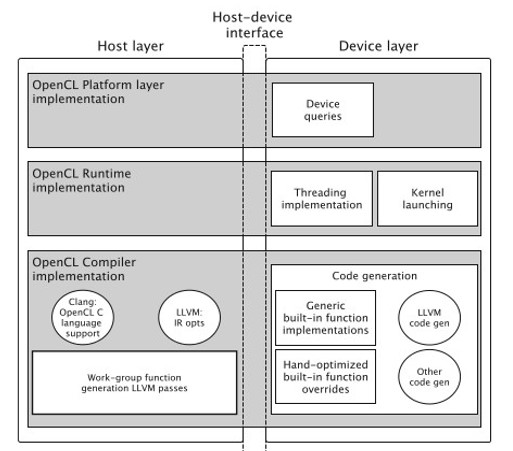
\includegraphics[width=1\textwidth]{soft_arch}
    \caption{POCL Software Framework}
    \label{fig:4_PM}
\end{figure}

Second, Device layer, which is dependent to the physical device, has default devices such as pthread, cuda, basic, ttasim and hsa. It can be found at /lib/CL/devices/ location in pocl. Device layer is responsible for code generation for the target, after performing device dependent optimization. OpenCL framework are C based implementation, which calls the function in device layer through generic host-device layer. For example, when global memory space is requested from application for buffer allocation, these queries are processed to device layer through host-device interface.

POCL software architecture offers easy portability for devices. The pthread device layer implementation can be ported for Symmetric Multi-Processing (SMP) systems that support pthread APIs in their operating system. Even ttasim device drivers can communicate and allocate buffers through DMA commands. Another main aspect of POCL is memory management for devices. They provide Bufalloc mechanism for memory allocation so that the buffers are used as a generic memory. The memory region is considered like a memory pools that the chunks of the region are returned based on the availability with every malloc call. 

\section{Platform Layer Implementation}
The platform name is called as Portable Computing Language with platform version as an OpenCL standard version and pocl release version. In OpenCL, we have a platform model to select the available number of devices in the system. Here, the platform layer of pocl queries the available number of devices through host-device layer. However, the device specific queries can be found in the device layer. POCL checks the environmental variable for enabled device. The software components of pocl may contain many OpenCL device implementation but the device can be enabled by environmental variable. This platform query can be found in /lib/CL/devices/device.c. The device specific information like global memory size, local memory varies from device to device. So, it is found under specific device names in basic devices directory, /lib/CL/devices/basic/. In addition, pocl also has device specific extra function calls to compute device. For example, In /lib/CL/devices/cpuinfo.c, it updates the number of parallel compute units or cores available for CPU parallel implementation.

\section{Portable kernel Compiler}
POCL provides an OpenCL C kernel compiler which it can parallelize the kernels to improve the performance of portability. It is based on Clang \cite{19} and LLVM \cite{20}. POCL kernel compiler’s compilation flow begins with parsing of OpenCL C kernel functions using Clang which produces LLVM Intermediate representations (IR). These LLVM IRs are used in pocl kernel compiler passes. Generally, the LLVM IR are the representation of single work-item of kernel functions. The execution of single work-item on the target device depends on the target model. If the device is designed for Single Program Multiple Data (SPMD) style, then the single work-item can be passed and the same applicable for other sets of data. In case of some GPU architecture, the same style is valid for Single Instruction Multiple Thread (SIMT) execution models, where each core of GPU receives the same instructions with same program counter value globally. 

To improve the performance portability, pocl host layer’s kernel compiler implementation can pack the OpenCL work-items into work-groups with synchronization barrier that can be mapped to the desirable parallel resources available in the target device. For example, when the target device is superscalar or Very Long Instruction Word (VLIW) architecture style, then it is efficient to unroll the parallel region of the work-items and schedule statically to multiple functional units. In other end, if work-groups are not feasible due to vectorization, POCL gives better way to avoid excessive divergence control flow by executing all the work-items serially using loops. POCL has built-in vectorized mathematical library in OpenCL C that can be linked with kernels. The work group function is passed to the assembler and code generator to get the executable kernel binary for target device. Also, these work group function possess a launcher function to execute in a heterogeneous environment where each device processes the launching request. The complete pocl kernel compiler flow is shown in the Figure \ref{fig:5_KCF} \cite{18}. 1. Compile Kernel by Clang 2. Linked with target-specific built-in functions such as sin, cos, etc. 3. Work-group Function Generation 4. Backend Optimization and Code Generation.
\begin{figure}[h]
    \centering
    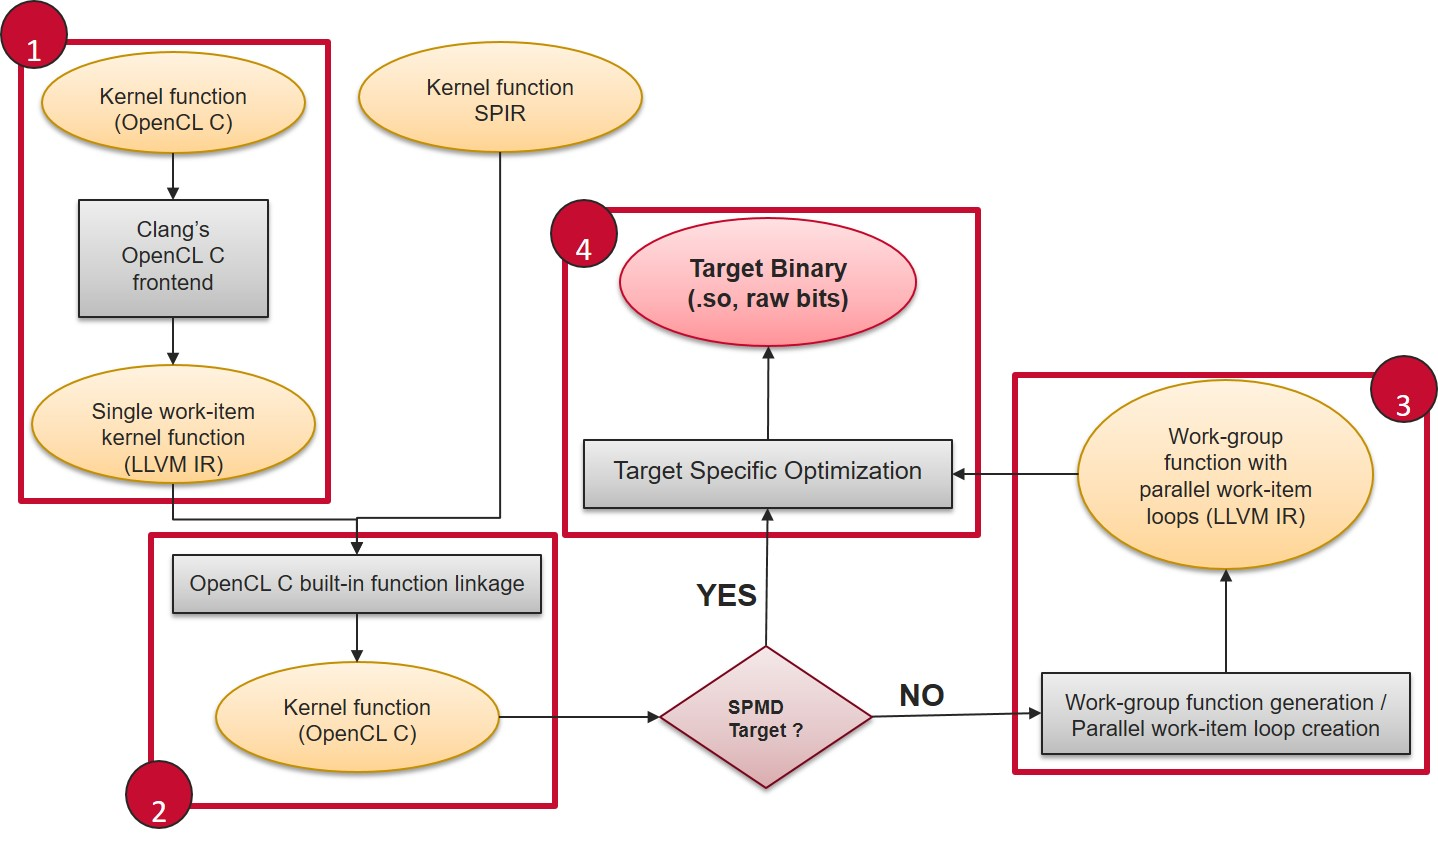
\includegraphics[width=1\textwidth]{POCL_COMPILATION_FLOW}
    \caption{POCL Kernel Compilation Flow}
    \label{fig:5_KCF}
\end{figure}

\section{Introducing new compute device to POCL}
The POCL Device layer should be included with following functionalities to add a new device. They are querying devices, managing memories, data transfers and generation of machine codes. In this context, we refer device layer as ‘basic’ device, which is a demo CPU device layer implementation. This basic device can be customized to create support for new OpenCL standard device.

\subsection{Device Query}
The host app requires the available number of devices and its device pointer for further OpenCL API calls. The Initialization function for all device types count the number of available devices using pocl\_basic\_probe() function in the device layer implementation. From user space, we can export the available device using POCL\_DEVICES with device name. When the probe function of a respective device type matches with the available environmental device name, then the devices are accounted. We can also include multiple accelerators for a device type by introducing a sysfs interface \cite{14}, which can be probed from device layer.

\subsection{Memory Management}
Using clCreateBuffer OpenCL API, read and write mode memory objects can be created for a given size. The current implementation of device layer creates memory objects in host CPU, which is  defined in pocl\_basic\_alloc\_mem\_obj(). To create memory object for an accelerator device, pocl\_basic\_alloc\_mem\_obj() should assign the memory object's mem\_ptr as a allocated memory address in the device. These memory objects are used to write and read data in device. The memory management for a new device is dependent on device's memory organization.

\subsection{Data Transfer}
The transfers are initiated by clEnqueueReadBuffer() and clEnqueueWriteBuffer() OpenCL APIs. These APIs push the read/write operations to command queue. pocl\_basic\_read() and pocl\_basic\_write() has device level definition in device layer. This can be integrated as an OpenCL Drivers with respective to device.

\subsection{Code Generation}
The conversion of kernel source code into machine code consists of the following steps.
\begin{itemize}
	\item POCL parses the kernel descriptions into LLVM IR using OpenCL C Frontend. This action is invoked inside clBuildProgram.c. The output representation is a description for single work item.
	\item Based on the targets (SPMD or not), single-work items needs to be converted to work-group function using clEnqueueNDRangeKernel().
	\item LLVM IR is converted into machine code from device layer using llvm\_codegen(). llvm\_codegen() uses the pocl's LLVM APIs to convert work group functions into native machine code. The LLVM API calls can be found in pocl\_llvm\_api.c.
	\item Allocating memory for kernel in device and writing machine code into device are defined inside pocl\_basic\_run().
\end{itemize}
To support code generation for a new device, we can reuse the OpenCL C Frontend to generate LLVM IR and the device's LLVM backend must be integrated to llvm\_codegen().
